This chapter will review the design of the design review application, with special emphasis on three subjects: The functional requirements, the gesture scheme and the technology choices.
The functional requirements of the application will be laid out through several use cases. These describe the different functionality by statements on the form
"the user should be able too.." (e.g.~move or place an annotation). The gesture scheme is discussed next, and is a definition of the different gestures
a user can perform, how they are performed and what action they should result in. Lastly, this chapter will cover the different technology choices, more specifically: What
software framework to use, what virtual reality HMDs to target and what gesture recognition system to utilize. 

%\section{The core functionality} 
In section~\vref{sec:initial_design} the fundamental design ideas for the virtual reality design review application was discussed. 
To ensure that such an application could change the work flow of DNV GL's design reviews, multiple design aspects should be met and a satisfactory infrastructure would need to be
set up. As this thesis' scope is limited to virtual reality and gesture recognition technology's role in such an application, several of the components necessary for
a satisfactory product will not be implemented to focus more one these aspects. The resulting implementation, which this design chapter outlines, will thus be more
a prototype or proof-of-concept of how virtual reality and gesture recognition technology can be used to interact and work with 3D models. 

\section{The Application's Functionality}
\import{}{2-application_functionality.tex}

\section{The Gestures}
\label{sec:gesture_design}
\import{../3-design/}{3-gesture-scheme.tex}

\section{Technology Choices}
\label{sec:design_choices}
There are several technology choices to make with regards to the implementation of the design review application.
These choices include programming framework or platform, what language to use, and what brand of gesture recognition technology and
virtual reality technology to use. Its also important to make sure that these choices are as compatible with each other as possible.

% A major decision is what programming framework to use. In the implementation the Unity game engine will be utilized.
\subsection{Software Framework}
Selecting a suitable software framework can save a lot of time during implementation, and simplify a lot of the implementation details. 
If the framework is popular, several other relevant frameworks, SDKs and libraries might also have integration or explicit support for it, 
meaning one can be fairly confident that the two are compatible and working well together. 
As the design review application will primarily be dealing with rendering, calculations and manipulation of 3D objects, using a game engine - which is specifically tailored for handling
these topics - is an interesting option.
A game engine is a software framework, usually designed for development of video games. 
The core functionality of a game engine typically includes a rendering engine, a physics engine (at least providing collision detection), sound, scripting, 
animation, networking, streaming, memory management, and threading~\citep{Gregory2014}. As game engines are created to enable development of complex 
3D environments and contain many of the facilities necessary for the application use cases outlined above, they provide a good foundation for the implementation.
Even though several game developers develops their own proprietary game engines, which are kept strictly private to the company, there are several commercially available ones 
as well. The biggest of these today is arguably the Unity and the Unreal engines, both with broad support from a number of third party vendors. 
This is a great benefit for the implementation phase as support for our choice of virtual reality and gesture recognition technology "straight out of the box" 
will ease the development process.

Of these two popular game engines the Unity engine was selected as the software platform. This was both a request from DNV GL, 
as they have experience with it from other projects, and also enabled the reuse of an asset bundle - containing a tanker model (see figure~\vref{fig:tank_outside}) 
- from one of their other projects.
The Unity engine and its central concepts will be discussed in chapter~\vref{chapter:technical}.

\begin{figure}%[h!] %[H]
	\frame{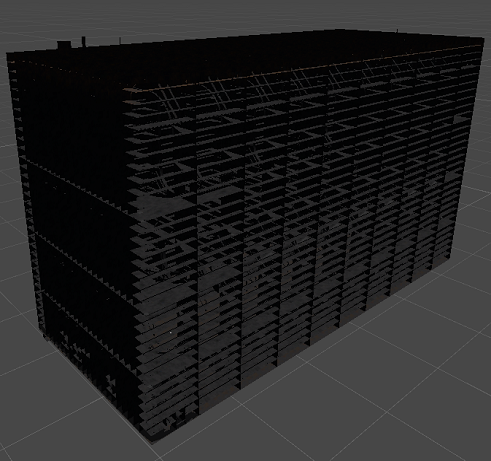
\includegraphics[width=0.5\linewidth]{pictures/screenshots/tank_back.png}}
	\frame{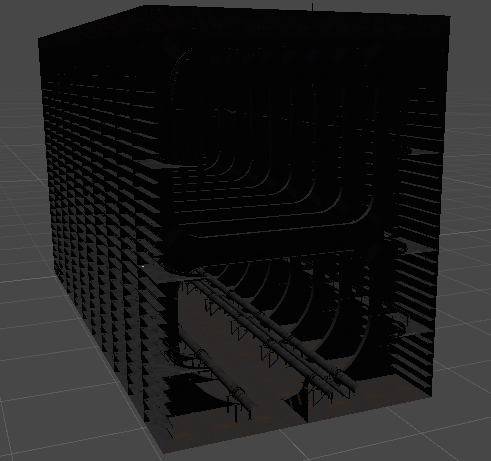
\includegraphics[width=0.5\linewidth]{pictures/screenshots/tank_half_profile.png}}
	\caption[The oil tanker model provided by DNV GL.]{The oil tanker model provided by DNV GL. This was used as a default model in the design review application.}
	\label{fig:tank_outside}
\end{figure} 

\subsection{Virtual Reality Device}
The virtual reality design review application should be targeted toward usage with modern head-mounted VR devices.
As DNV GL possesses a HTC Vive, and this HMD will be used in test sessions with potential end-users after implementation, 
the application should work optimally with it. However, as this device is only available at their facilities, and not during development, support 
should also be added for Oculus Rift DK2\footnote{The Development Kit 2, a predecessor or DK1, releases in 2014} as it is available via Simula Research Laboratory.
As these two HMDs have separate SDKs and runtime environment, support for them have to be added individually. 
Luckily, Unity 5 supports both HMDs natively (i.e "out-of-the-box") by enabling the project specific setting "Virtual Reality Supported", 
so adding the basic VR functionality - such as camera rotation on head turn - is trivial. 
Implementing support for both these virtual reality headsets also enable a comparison of their performance in the application, to, at least, indicate whether 
one HMD perform better than the other. 

\subsection{Gesture Recognition Device}
\label{sec:design_leapmotion}
When deciding on what vision-based gesture recognition system to utilize the Leap Motion Controller, from the company Leap Motion Inc., was chosen.
The primary reasons behind this choice were as follows: 
\begin{itemize}
    \item It is a vision-based gesture recognition device that focuses only on hand gestures, and should thus offer better hand-tracking capabilities than devices that focus 
          on the whole body (such as Microsoft's Kinect~\citep{Zhang2012}).
    \item It has been relatively well received by several evaluations and has been reported to have a higher accuracy than similar systems in the same price range
            (see evaluations by~\citet{Weichert2013} and~\citet{Guna2014}).
    \item It utilizes stereoscopic vision, which - as discussed in section~\vref{sec:vision_based_comparison} - is arguably the most promising vision-based technology.
    \item It is both relatively small (the size of a matchbox) and cheap (about 70 euro at the time of writing), which makes it optimal for usage in regular work spaces. 
    \item It has a well-documented API\footnote{Application Programming Interface: A defined set of high-level functions or abstractions other software can utilize.}, which 
          supports multiple programming languages. This API is reviewed in chapter~\ref{chapter:technical}.
\end{itemize}

The Leap Motion controller also have software components tailored for use with the Unity Engine, which also made it a convenient choice. 
These components ensure that the usage of the Leap Motion Controller in the design review application is conducted after Leap Motion's best practices. 

\section{Summary and Final Thoughts}
With these software frameworks we get several pre-made software components, which enables us to focus more on the application specifics during the implementation phase.
The high fidelity tanker model, provided by DNV GL, gives us a default model we can prototype all functionality on, before generalizing the application to accept other models as
well. This generalization should be done before the application is used in any professional capacity, but it is outside the scope of this thesis. 
In addition to the model, the SDK and runtime libraries of the virtual reality vendors can be added to the project, and (presumably) work without any custom code. 
The design review application should enable the user to easy switching between these two virtual reality headsets and a desktop mode, for use without a virtual reality headset.
The Leap Motion Controller SDK and runtime library (called Orion) also provides some standard assets we can use in the implementation. 
The most useful of these assets include hand models, API-scripts (to retrieve information from the device) and detectors, which is used to recognize gestures. 
These Leap Motion components are covered more thoroughly in chapter~\ref{chapter:technical}.

Before the implementation is described and documented in chapter~\ref{chapter:implementation}, we will do a technical review in chapter~\ref{chapter:technical}. 
The technical review will expand upon the framework and devices choices we did in section~\ref{sec:design_choices}, and introduce some of their core concepts. 
This should again lay the ground work for understanding the implementation, which is documented in chapter~\ref{chapter:implementation}.


% Carsten:
% Write a conclusion for this chapter.
% I recommend that this contains a requirement for understanding the rendering engine and the user interaction in more detail.
% You could then write a single chapter that comprises as 2 subsections, 
% first (a) new text introducing Unity, because that is dearly missed, (b) the old chapter 4 text about the Leap motion. 

% \section{Functionality limitations}
% \subsection{Handling textual input with gestures}
% \subsection{User gesture calibration}
% \subsection{Saving annotation to a database}
% \subsection{Exposing annotation to web servers}
% \subsection{Annotation time-lines}

% \section{Challenges with VR and GRT} 
% Problems with using VR + e.g Leap over mouse + keyboard + display. E.g:

% \subsection{The "writing issue"}
% Virtual keyboards are bad. 
% Regular keyboards are impractical. 
% See "ideer til masteroppgaven.txt"
% 
% \subsection{Challenges in "designing" gesture schemes}
% People have different preferences. Have intuitive gestures. Have gestures that is not too
% fatiguing. Have gesture with high precision and recall (F-score) (high TP and TN. Low FP, FN).
% Have a system that doesnt mistake one gesture for another.
% 
% \subsubsection{Fixes?}
% User-gesture calibration. 
% 
% \section{Related work}

